% Chapter 1: Sets (notes 1.1-1.5 and 2.5.1). Fragment: \input from the main file.
% Helper macros use the \sets prefix so they can't clash with other chapters.
\newcommand{\setsP}{\mathcal{P}}
\newcommand{\setsSt}{\mathrel{|}}
% \setsVenn{xshift}{fill commands}{label}: one two-circle Venn diagram inside a universe box
\newcommand{\setsVenn}[3]{%
  \begin{scope}[xshift=#1]
    \path[use as bounding box] (-0.2,-1.55) rectangle (2.5,1.1);
    #2
    \draw (-0.1,-0.95) rectangle (2.4,0.95);
    \node[font=\scriptsize,anchor=north west,inner sep=1.5pt] at (-0.1,0.95) {$\mathcal{U}$};
    \draw (0.8,0) circle (0.62);
    \draw (1.5,0) circle (0.62);
    \node[font=\scriptsize] at (0.45,0) {$A$};
    \node[font=\scriptsize] at (1.85,0) {$B$};
    \node[font=\small] at (1.15,-1.3) {#3};
  \end{scope}}

\section{Sets}

Almost everything in this course is built out of sets, and almost every set question on Test~1 comes down to one move: asking whether a specific thing is a member of a specific set. If you get good at that one move, the operations, subsets and power sets stop being separate topics. They're all membership questions in different clothes.

% ------------------------------------------------------------------
\subsection{Membership is the whole story}

Here's a set: $M=\{a,\ \{a\},\ \{b,c\}\}$. How many members does it have? Three. The letter $a$, the set $\{a\}$, and the set $\{b,c\}$. Is $b$ a member of $M$? No. The letter $b$ shows up on the page, but it's sitting inside one of $M$'s members, not in $M$'s own list.

That's the mindset for this whole chapter. A set is defined by which things are its members, and nothing else. There's no first member, no second member, no ``how many times'' a member appears. Something is either a member or it isn't.

\begin{notebox}
\textbf{Set, member.} A set is a thing that has members. $x\in A$ means ``$x$ is a member of $A$''; $x\notin A$ means it isn't. Two sets are the same set exactly when they have the same members.

\textbf{Set-list notation.} List the members between curly braces: $\{1,2,3\}$. Round parentheses or square brackets do \emph{not} make a set.

\textbf{Empty set.} The set with no members, written $\varnothing$ or $\{\}$.
\end{notebox}

Two consequences fall straight out of the definition. Order doesn't matter, so $\{3,1,2\}=\{1,2,3\}$. Repeats don't matter either, so $\{3,1,1,2\}=\{1,2,3\}$: writing $1$ twice just says ``$1$ is a member'' twice. When you write an answer in set-list notation, write each member once anyway. Repeats in an answer look like you think they count.

\textbf{Worked example.} With $M=\{a,\{a\},\{b,c\}\}$:
\begin{itemize}
  \item $a\in M$: yes, it's listed.
  \item $\{a\}\in M$: yes, also listed. So $M$ has both $a$ and $\{a\}$ as members, and they're different members.
  \item $\{b,c\}\in M$: yes.
  \item $b\in M$: no. It's a member of a member, which doesn't count.
  \item $\varnothing\in M$: no. Nothing in the list is the empty set.
\end{itemize}
For a set written in set-list form, membership is the dumbest possible check: is it literally one of the listed items? No other test applies.

\textbf{Where people slip.}
\begin{itemize}
  \item Reading ``$b$ appears somewhere inside the braces'' as ``$b\in M$''. Only the top-level items are members.
  \item Treating $\varnothing$ as a member of every set. It isn't (more on why people think so in \S\ref{sets:ein}).
  \item Writing $\epsilon$ for $\in$. In this course $\varepsilon$ means the empty string, so keep the symbols apart.
\end{itemize}

% ------------------------------------------------------------------
\subsection{Set-builder notation}

Listing members breaks down fast. You can't list the even integers, and ``$\{3,4,6,8,12,\dots\}$'' makes the reader guess the pattern. Set-builder notation gives a recipe instead: a template on the left of the bar, and the conditions the template's variables must meet on the right.

\begin{notebox}
\textbf{Set-builder notation.} $\{\text{template}\setsSt\text{condition}\}$ is the set of everything you can get by plugging values that meet the condition into the template, and nothing else. Read the bar as ``such that'' or ``where''.
\end{notebox}

So $\{3k+1\setsSt k\in\mathbb{N}\}=\{1,4,7,10,\dots\}$. To decide whether some $x$ is a member, you try to \emph{match} $x$ to the template with legal values. One successful match is enough, so a membership claim like this is really a ``there exists'' claim.

\textbf{Worked example.} Let $F=\{3k+1\setsSt k\in\mathbb{N}\}$.
\begin{itemize}
  \item $10\in F$? Set $3k+1=10$, so $k=3$, and $3\in\mathbb{N}$. Yes.
  \item $0\in F$? We'd need $3k+1=0$, so $k=-\tfrac13$, which isn't a natural number. No other $k$ works, so no.
  \item $-2\in F$? We'd need $k=-1\notin\mathbb{N}$. No. But change the condition to $k\in\mathbb{Z}$ and the answer flips to yes. The condition is part of the definition.
\end{itemize}

Sometimes nothing meets the condition. $\{x\in\mathbb{N}\setsSt x<0\}$ has no members, so it's just $\varnothing$ written in a roundabout way.

You'll also see the variable's home set written on the left, as in $\{x\in\mathbb{N}\setsSt x<0\}$. That means the same as $\{x\setsSt x\in\mathbb{N}\text{ and }x<0\}$.

\textbf{Where people slip.}
\begin{itemize}
  \item Finding one value that \emph{doesn't} match and concluding ``not a member''. You need to show that \emph{no} legal value matches.
  \item Forgetting the condition. Plugging $k=-1$ into $3k+1$ gives $-2$, but $-1$ isn't allowed when $k\in\mathbb{N}$.
\end{itemize}

% ------------------------------------------------------------------
\subsection{The number sets}

You'll use these constantly as universes and as conditions in set-builder notation.

\begin{center}
\begin{tabularx}{\linewidth}{@{}lL@{}}
\toprule
\textbf{Set} & \textbf{What's in it}\\
\midrule
$\mathbb{N}$ & natural numbers $\{0,1,2,3,\dots\}$. In this course $0\in\mathbb{N}$, no exceptions.\\
$\mathbb{Z}$ & integers $\{\dots,-2,-1,0,1,2,\dots\}$\\
$\mathbb{Q}$ & rationals: $\{\frac pq\setsSt p\in\mathbb{Z}\text{ and }q\in\mathbb{Z}\text{ and }q\neq0\}$\\
$\mathbb{R}$ & reals: anything on the number line, any decimal expansion\\
\bottomrule
\end{tabularx}
\end{center}

The $\mathbb{Q}$ definition is set-builder notation, so the rule from the last section applies: the question is whether a number \emph{can be written} as an integer over a nonzero integer, not how it happens to be written right now. $\frac{0.5}{0.25}$ doesn't look like it qualifies, but it equals $\frac21$, so it's rational. $\sqrt9=\frac31$ is rational. $\frac{\pi}{2}$ is a ratio, but not of integers, and it can't be rewritten as one, so it isn't.

\textbf{Where people slip.} Leaving $0$ out of $\mathbb{N}$ because an older book did. Also: $\mathbb{N}\subseteq\mathbb{Z}\subseteq\mathbb{Q}\subseteq\mathbb{R}$, so every integer is rational. ``Rational'' doesn't mean ``has a fraction bar''.

% ------------------------------------------------------------------
\subsection{Union, intersection, difference, complement}

You probably learned these as ``smush the lists together'' and ``keep the overlap''. That works for small listed sets, but it falls apart once sets are defined by conditions. The definitions you'll actually use in proofs are membership tests: each operation says exactly when some $x$ is a member of the result.

\begin{notebox}
\textbf{Union.} $x\in A\cup B$ means $x\in A$ or $x\in B$ (or both).\\
\textbf{Intersection.} $x\in A\cap B$ means $x\in A$ and $x\in B$.\\
\textbf{Relative complement (difference).} $x\in A-B$ means $x\in A$ and $x\notin B$.\\
\textbf{Complement.} $x\in\overline{A}$ means $x\notin A$. This only makes sense once a universe $\mathcal{U}$ is fixed; then $\overline{A}=\{x\in\mathcal{U}\setsSt x\notin A\}$.
\end{notebox}

Notice that each operation is a logic connective in disguise: $\cup$ is ``or'', $\cap$ is ``and'', $-$ is ``and not'', and the overline is ``not''. That link is why the logic in \S\ref{logic:start} keeps coming back to sets.

\begin{figure}[H]
\centering
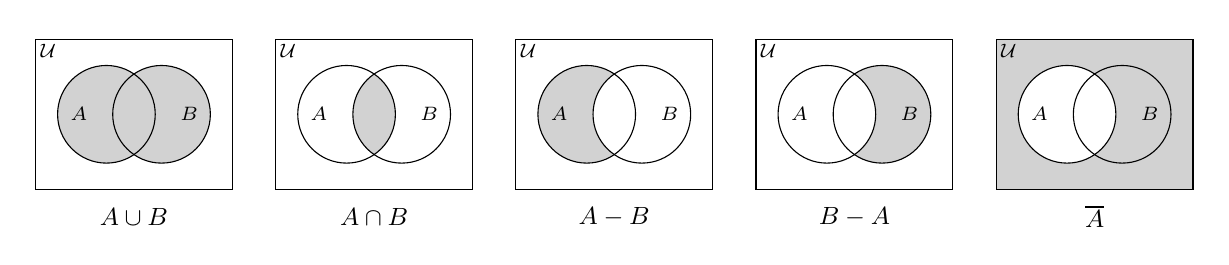
\begin{tikzpicture}[shade/.style={fill=gray!35}]
  \setsVenn{0cm}{\fill[shade] (0.8,0) circle (0.62); \fill[shade] (1.5,0) circle (0.62);}{$A\cup B$}
  \setsVenn{3.05cm}{\begin{scope}\clip (0.8,0) circle (0.62); \fill[shade] (1.5,0) circle (0.62);\end{scope}}{$A\cap B$}
  \setsVenn{6.1cm}{\fill[shade] (0.8,0) circle (0.62); \fill[white] (1.5,0) circle (0.62);}{$A-B$}
  \setsVenn{9.15cm}{\fill[shade] (1.5,0) circle (0.62); \fill[white] (0.8,0) circle (0.62);}{$B-A$}
  \setsVenn{12.2cm}{\fill[shade] (-0.1,-0.95) rectangle (2.4,0.95); \fill[white] (0.8,0) circle (0.62);}{$\overline{A}$}
\end{tikzpicture}
\caption{The shaded region is everything that passes the membership test. $A-B$ and $B-A$ are different regions, and $\overline{A}$ fills the rest of the universe box, so it changes if the box changes.}
\end{figure}

\textbf{Worked example.} Take $\mathcal{U}=\{0,1,\dots,9\}$, $A=\{1,2,3,4\}$, $B=\{3,4,5,6\}$.
\begin{itemize}
  \item $A\cup B=\{1,2,3,4,5,6\}$.
  \item $A\cap B=\{3,4\}$.
  \item $A-B=\{1,2\}$. Go through $A$ member by member and drop anything in $B$.
  \item $B-A=\{5,6\}$. Different set. Difference isn't symmetric, the same way $7-3\neq3-7$.
  \item $\overline{A}=\{0,5,6,7,8,9\}$. Now shrink the universe to $\{1,\dots,6\}$ and $\overline{A}$ becomes $\{5,6\}$. Same $A$, different answer.
\end{itemize}

\textbf{Where people slip.}
\begin{itemize}
  \item Computing $B-A$ when asked for $A-B$. Always start from the \emph{left} set.
  \item Taking a complement without writing down the universe first. If a problem gives you $\overline{A}$, find the stated universe before doing anything else.
  \item Writing $A\land B$ when you mean $A\cap B$. Connectives join statements; $\cap$ and $\cup$ join sets. ``$x\in A\cap B$'' is fine, ``$x\in A\land B$'' is a type error.
\end{itemize}

% ------------------------------------------------------------------
\subsection{Cardinality}

\begin{notebox}
\textbf{Cardinality.} For a finite set $A$, $|A|$ is the number of members of $A$.
\end{notebox}

Count distinct members only, and count members, not symbols:
\begin{itemize}
  \item $|\{3,1,1,2\}|=3$, since the repeat collapses.
  \item $|\{\{1,2,3\}\}|=1$. One member, which happens to be a set with three members.
  \item $|\varnothing|=0$ and $|\{\varnothing,\{\varnothing\}\}|=2$.
  \item $|\{x\in\mathbb{Z}\setsSt 0<x^2<5\}|=4$, because the members are $-2,-1,1,2$.
\end{itemize}
For infinite sets like $\mathbb{Z}$, just say the set is infinite. Comparing sizes of infinite sets is a much later topic.

\textbf{Where people slip.} Counting the members of the members. In $\{\{1,2,3\}\}$ the inner $1,2,3$ are one level too deep to count.

% ------------------------------------------------------------------
\subsection{Subsets, proper subsets, set equality}

Membership relates a thing to a set. Subset relates a set to a set, and it's a statement about all of the first set's members at once.

\begin{notebox}
\textbf{Subset.} $A\subseteq B$ means every member of $A$ is a member of $B$. (Also written $B\supseteq A$, ``$B$ is a superset of $A$''.)\\
\textbf{Proper subset.} $A\subsetneq B$ means $A\subseteq B$ and $A\neq B$.\\
\textbf{Set equality.} $A=B$ exactly when $A\subseteq B$ and $B\subseteq A$.
\end{notebox}

The symbol $\subseteq$ looks like $\leq$ on purpose: every set is a subset of itself, the same way $5\leq5$. Avoid $\subset$ entirely. Some people read it as $\subseteq$ and others as $\subsetneq$.

Because ``every member'' is a universal claim, the two directions of proof are lopsided:
\begin{itemize}
  \item To show $A\subseteq B$, you have to cover \emph{every} member of $A$. For a short list, check them one by one. For a set-builder set, take an arbitrary member and argue it lands in $B$.
  \item To show $A\not\subseteq B$, you need \emph{one} member of $A$ that isn't in $B$. Name it.
\end{itemize}

\textbf{Worked example.}
\begin{itemize}
  \item $\{2,3\}\subseteq\{1,2,3\}$: both $2$ and $3$ are listed on the right. Since the sets differ, it's also $\{2,3\}\subsetneq\{1,2,3\}$.
  \item $\{0,5\}\not\subseteq\{n^2\setsSt n\in\mathbb{Z}\}$: the witness is $5$. It's in the left set, and $n^2=5$ has no integer solution.
  \item $\{n\in\mathbb{Z}\setsSt 0<n<4\}=\{1,2,3\}$. Left to right: an integer strictly between $0$ and $4$ is $1$, $2$ or $3$. Right to left: each of $1,2,3$ is an integer strictly between $0$ and $4$.
  \item $\{1,2\}$ and $\{2,3\}$: neither is a subset of the other ($1$ blocks one direction, $3$ the other). Unlike numbers, two sets don't have to be comparable.
\end{itemize}

One more structural fact: $\subseteq$ chains. If $A\subseteq B$ and $B\subseteq C$, then $A\subseteq C$. Membership does not chain: $1\in\{1\}$ and $\{1\}\in\{\{1\}\}$, but $1\notin\{\{1\}\}$, because the only member of $\{\{1\}\}$ is the set $\{1\}$.

\textbf{Where people slip.}
\begin{itemize}
  \item Proving $A\subseteq B$ by checking a couple of examples. That's evidence, not a proof, unless the examples are all of $A$'s members.
  \item Answering ``no'' to a subset question without naming the member that breaks it.
  \item Writing $\{1,2\}\subsetneq\{1,2\}$. Proper means the sets have to differ.
\end{itemize}

% ------------------------------------------------------------------
\subsection{\texorpdfstring{$\in$ versus $\subseteq$}{Member versus subset}}\label{sets:ein}

This is the single most common way to lose points on set questions, and the cause is a picture most people carry around: a set as a container, with stuff ``in'' it. The trouble is that ``in'' (and ``contains'') covers two different relationships. ``$\{1\}$ is in $\{1,2\}$'' could mean member or subset, and only one of those is true. So stop saying ``in'' and ``contains'' when you study. Say ``member of'' or ``subset of'', and the right answer usually becomes obvious.

\begin{figure}[H]
\centering
\begin{tikzpicture}[item/.style={draw,rectangle,inner sep=3pt,minimum height=1.5em,font=\small},
                    atom/.style={inner sep=2pt,font=\small}]
  % left panel: membership
  \begin{scope}
    \node[draw,rounded corners=3pt,minimum width=5.6cm,minimum height=2.3cm] (M1) at (0,0) {};
    \node[anchor=north west,font=\small] at (M1.north west) {$M$};
    \node[atom] (a1) at (-1.8,0.1) {$a$};
    \node[item] (A1) at (-0.3,0.1) {$a$};
    \node[item,hl] (BC1) at (1.5,0.1) {$b\quad c$};
    \node[font=\scriptsize] (bnote) at (1.5,-0.85) {$b$ is two levels down};
    \node[lbl,align=center] at (0,-1.75) {$\in$: point at \emph{one} item.\\ $\{b,c\}\in M$ \quad but \quad $b\notin M$};
  \end{scope}
  % right panel: subset
  \begin{scope}[xshift=7.4cm]
    \node[draw,rounded corners=3pt,minimum width=5.6cm,minimum height=2.3cm] (M2) at (0,0) {};
    \node[anchor=north west,font=\small] at (M2.north west) {$M$};
    \node[atom] (a2) at (-1.8,0.1) {$a$};
    \node[item] (A2) at (-0.3,0.1) {$a$};
    \node[item] (BC2) at (1.5,0.1) {$b\quad c$};
    \draw[dashed,rounded corners=6pt] ($(a2.south west)+(-0.25,-0.3)$) rectangle ($(A2.north east)+(0.25,0.3)$);
    \node[lbl,align=center] at (0,-1.75) {$\subseteq$: pick \emph{some} items, put them in a new box.\\ $\{a,\{a\}\}\subseteq M$};
  \end{scope}
\end{tikzpicture}
\caption{$M=\{a,\{a\},\{b,c\}\}$ drawn with a box for every pair of braces. Each inner box is a single item of $M$. A member is one item; a subset is a new box whose items all come from $M$'s items.}
\end{figure}

The working test for each:
\begin{itemize}
  \item ``$x\in Y$?'' Is $x$ one of $Y$'s items? Nothing else matters.
  \item ``$X\subseteq Y$?'' First, $X$ has to be a set. Then: is each item of $X$ one of $Y$'s items?
\end{itemize}

\textbf{Worked example.} Still with $M=\{a,\{a\},\{b,c\}\}$:
\begin{itemize}
  \item $\{a\}\in M$ and $\{a\}\subseteq M$. Both! It's listed, \emph{and} its only member $a$ is listed.
  \item $\{b,c\}\in M$, but $\{b,c\}\not\subseteq M$, because $b\notin M$.
  \item $\{b\}\notin M$ and $\{b\}\not\subseteq M$. Neither.
  \item $\varnothing\notin M$, but $\varnothing\subseteq M$.
\end{itemize}

That last pair is the classic. The empty set is a subset of every set: to break $\varnothing\subseteq M$ you'd need a member of $\varnothing$ that isn't in $M$, and $\varnothing$ has no members to offer. (That's vacuous truth, covered in the logic chapter.) But $\varnothing$ is a member of a set only if it's actually listed. The two facts get blurred into ``the empty set is in every set'', and that sentence is half wrong.

\textbf{Where people slip.}
\begin{itemize}
  \item Concluding $\{1,2,3\}\in\{0,1,2,3\}$ because ``all of its members are in there''. That argument proves $\subseteq$, never $\in$.
  \item Writing $2\subseteq\{1,2\}$. A number isn't a set, so it can't be a subset of anything. Write $\{2\}\subseteq\{1,2\}$ or $2\in\{1,2\}$.
\end{itemize}

% ------------------------------------------------------------------
\subsection{\texorpdfstring{Wrapping in braces: $1$ vs $\{1\}$, $\varnothing$ vs $\{\varnothing\}$}{Wrapping in braces}}

Every pair of braces makes a new object. $\{1\}$ is not a fancier way to write $1$; it's a set whose one member is the number $1$. Same for $\varnothing$ and $\{\varnothing\}$: the first is an empty box, the second is a box with one item, and that item happens to be an empty box.

\begin{figure}[H]
\centering
\begin{tikzpicture}[set/.style={draw,rectangle,inner sep=4pt,minimum height=1.6em,minimum width=1.6em,font=\small}]
  \node[font=\small] (n1) at (0,0) {$1$};
  \node[set] (s1) at (2.0,0) {$1$};
  \node[set] (e0) at (4.4,0) {};
  \node[set,minimum width=2.4em,minimum height=2.4em] (e1) at (6.6,0) {};
  \node[set,minimum width=0.9em,minimum height=0.9em,inner sep=0pt] at (e1) {};
  \node[set,minimum width=5.0em,minimum height=2.4em] (e2) at (9.6,0) {};
  \node[set,minimum width=0.9em,minimum height=0.9em,inner sep=0pt] at ($(e2)+(-0.45,0)$) {};
  \node[set,minimum width=1.6em,minimum height=1.6em,inner sep=0pt] (inner) at ($(e2)+(0.45,0)$) {};
  \node[set,minimum width=0.6em,minimum height=0.6em,inner sep=0pt] at (inner) {};
  \foreach \n/\t/\c in {n1/{$1$}/{a number},s1/{$\{1\}$}/{1 member},e0/{$\varnothing$}/{0 members},e1/{$\{\varnothing\}$}/{1 member},e2/{$\{\varnothing,\{\varnothing\}\}$}/{2 members}}
    \node[font=\small,align=center] at ($(\n)+(0,-1.0)$) {\t\\[-1pt]\footnotesize\c};
\end{tikzpicture}
\caption{Each box is one pair of braces. Count a set's members by counting the items directly inside its outer box.}
\end{figure}

Facts worth having cold:
\begin{itemize}
  \item $1\neq\{1\}$. One is a number, the other a set.
  \item $1\in\{1\}$, $\{1\}\in\{\{1\}\}$, but $1\notin\{\{1\}\}$.
  \item $\{1\}\subseteq\{1,2\}$ but $\{1\}\notin\{1,2\}$.
  \item $|\varnothing|=0$ but $|\{\varnothing\}|=1$. So $\{\varnothing\}\neq\varnothing$.
  \item $\varnothing\in\{\varnothing\}$ and $\varnothing\subseteq\{\varnothing\}$. Both, for different reasons.
\end{itemize}

\textbf{Where people slip.} Writing an answer like $A\cap B=3$ when the answer is the set $\{3\}$. An operation on sets always gives a set, even when it has one member.

% ------------------------------------------------------------------
\subsection{Power sets}

\begin{notebox}
\textbf{Power set.} $\setsP(A)=\{B\setsSt B\subseteq A\}$, the set of all subsets of $A$.\\
For finite $A$, $|\setsP(A)|=2^{|A|}$.
\end{notebox}

Read the definition as a membership test, because that's how you'll use it: $X\in\setsP(A)$ means exactly $X\subseteq A$. Every question of the form ``is this in the power set?'' turns into a subset question.

To list $\setsP(A)$ without missing anything, go by size: the empty set, then all one-member subsets, then all two-member subsets, and so on up to $A$ itself.

\begin{figure}[H]
\centering
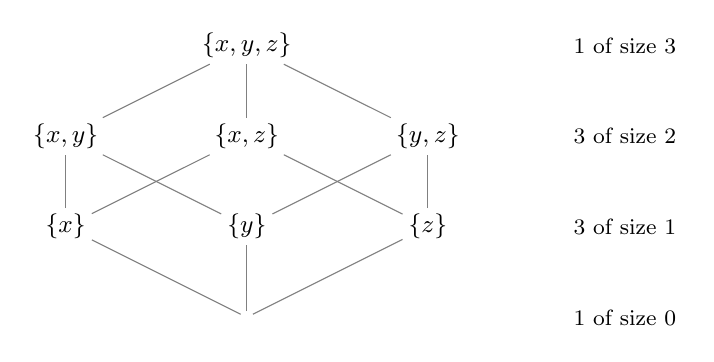
\begin{tikzpicture}[ps/.style={inner sep=2pt,font=\small},x=2.3cm,y=1.15cm]
  \node[ps] (e)   at (0,0)  {$\varnothing$};
  \node[ps] (x)   at (-1,1) {$\{x\}$};
  \node[ps] (y)   at (0,1)  {$\{y\}$};
  \node[ps] (z)   at (1,1)  {$\{z\}$};
  \node[ps] (xy)  at (-1,2) {$\{x,y\}$};
  \node[ps] (xz)  at (0,2)  {$\{x,z\}$};
  \node[ps] (yz)  at (1,2)  {$\{y,z\}$};
  \node[ps] (xyz) at (0,3)  {$\{x,y,z\}$};
  \foreach \a/\b in {e/x,e/y,e/z,x/xy,x/xz,y/xy,y/yz,z/xz,z/yz,xy/xyz,xz/xyz,yz/xyz}
    \draw[gray] (\a) -- (\b);
  \foreach \yy/\c in {0/1,1/3,2/3,3/1}
    \node[font=\footnotesize,anchor=west] at (1.75,\yy) {\c\ of size \yy};
\end{tikzpicture}
\caption{All eight members of $\setsP(\{x,y,z\})$. A line joins two subsets when the upper one adds exactly one member. Row counts $1+3+3+1=8=2^3$.}
\end{figure}

Why $2^{|A|}$? Building a subset means making one yes/no decision per member of $A$: in or out. Three members, three independent binary choices, $2\cdot2\cdot2=8$ subsets. It's the same count as the rows of a truth table with three variables, and that's not a coincidence.

\textbf{Worked example.}
\begin{itemize}
  \item $\setsP(\{x,y,z\})=\{\varnothing,\{x\},\{y\},\{z\},\{x,y\},\{x,z\},\{y,z\},\{x,y,z\}\}$. Both $\varnothing$ and the whole set are always in there.
  \item $\setsP(\varnothing)=\{\varnothing\}$. The empty set has exactly one subset (itself), so $|\setsP(\varnothing)|=1=2^0$.
  \item $|\setsP(\setsP(\{1\}))|$: $\setsP(\{1\})=\{\varnothing,\{1\}\}$ has 2 members, so the answer is $2^2=4$.
\end{itemize}

\textbf{Where people slip.}
\begin{itemize}
  \item Writing $1\in\setsP(\{1,2\})$. Members of a power set are \emph{sets}. The member is $\{1\}$.
  \item Claiming $A\subseteq\setsP(A)$. Usually false: the members of $A$ are things like numbers, the members of $\setsP(A)$ are sets. What's true is $A\in\setsP(A)$.
  \item Forgetting $\varnothing$ or $A$ itself when listing, then getting $2^n-1$ or $2^n-2$.
\end{itemize}

% ------------------------------------------------------------------
\subsection{Practice}

None of these come from homework. Try each one cold before you look at the answers; the point is to find out what you can do with nothing in front of you.

\begin{enumerate}[label=\textbf{\arabic*.},leftmargin=1.8em,itemsep=0.35em]
  \item Let $P=\{2,\{2\},\{2,3\},\varnothing\}$. For each $x$ below, say whether $x\in P$, whether $x\subseteq P$, both, or neither:\\
  (a) $\varnothing$ \quad (b) $\{2\}$ \quad (c) $2$ \quad (d) $\{2,3\}$ \quad (e) $\{\{2\}\}$ \quad (f) $\{3\}$
  \item Universe $\mathcal{U}=\{0,1,\dots,11\}$. Let $E=\{n\in\mathcal{U}\setsSt n\text{ is even}\}$ and $T=\{3k\setsSt k\in\mathbb{N}\text{ and }3k\leq 11\}$. Write in set-list notation: $E\cap T$, $T-E$, $E-T$, $\overline{E\cup T}$. Then compute $\overline{E}\cap\overline{T}$ and compare it with $\overline{E\cup T}$.
  \item Let $W=\{k^2+1\setsSt k\in\mathbb{Z}\}$. Which of $10, 1, 3, 0, 26$ are members of $W$? Then let $H=\{\frac ab\setsSt a\in\mathbb{N}\text{ and }b\in\mathbb{N}\text{ and }b\neq0\}$. Is $0\in H$? Is $0.75\in H$? Is $-\frac23\in H$?
  \item Write $\{x\in\mathbb{Z}\setsSt x^2<10\}$ in set-list notation and give its cardinality. Do the same with $\mathbb{N}$ in place of $\mathbb{Z}$.
  \item Let $Y=\{a,\{b\}\}$. List $\setsP(Y)$. What is $|\setsP(\setsP(Y))|$? Is $\{b\}\in\setsP(Y)$? Is $\{\{b\}\}\in\setsP(Y)$?
  \item True or false, with a one-line reason each:\\
  (a) $\varnothing\subseteq\varnothing$ \quad (b) $\varnothing\in\varnothing$ \quad (c) $\varnothing\in\{\varnothing\}$\\ (d) $\{\varnothing\}\subseteq\varnothing$ \quad (e) $|\{\varnothing,\{\varnothing\}\}|=2$ \quad (f) $\setsP(\varnothing)=\varnothing$
  \item (a) Find a nonempty set $A$ and a set $B$ with both $A\in B$ and $A\subseteq B$.\\
  (b) Find a set $x$ with both $x\in\{x\}$ and $x\subseteq\{x\}$.
  \item Let $A=\{1,2,3\}$ and $B=\{3,4\}$. Each statement has one mistake. Find it and fix it.\\
  (a) ``$\{3\}\in A$, because $3\in A$.'' \quad (b) ``$A-B=\{4\}$.'' \quad (c) ``$A\cap B=3$.''\\
  (d) ``$\varnothing\in A$, because the empty set is in every set.'' \quad (e) ``$\{1,2,3,3\}$ has four members.''
  \item (a) How many subsets of $\{1,2,3,4,5\}$ have $1$ as a member but not $2$?\\
  (b) How many proper subsets does $\{1,2,3,4,5\}$ have?
\\  (c) What is $|\setsP(\{1,2\})\cup\{1,2\}|$?
  \item Let $X=\{1,2\}$. True or false:\\ (a) $X\in\setsP(X)$ \quad (b) $X\subseteq\setsP(X)$ \quad (c) $\{X\}\subseteq\setsP(X)$\\ (d) $\setsP(X)\cap X=\varnothing$ \quad (e) $\varnothing\in\setsP(X)\cap X$
  \item True or false, with justification:\\
  (a) $\{n\in\mathbb{Z}\setsSt n^2=n\}=\{0,1\}$ \quad
  (b) $\{3n+1\setsSt n\in\mathbb{Z}\}=\{3n-2\setsSt n\in\mathbb{Z}\}$\\
  (c) $\{n^2\setsSt n\in\mathbb{N}\}\subsetneq\mathbb{N}$ \quad
  (d) $\{3n+1\setsSt n\in\mathbb{N}\}=\{3n-2\setsSt n\in\mathbb{N}\}$
\end{enumerate}

% ------------------------------------------------------------------
\subsection{Answers}

Every answer here was checked by brute force.

\begin{enumerate}[label=\textbf{\arabic*.},leftmargin=1.8em,itemsep=0.45em]
  \item The members of $P$ are exactly the four listed items: $2$, $\{2\}$, $\{2,3\}$, $\varnothing$.
  \begin{itemize}
    \item (a) $\varnothing$: both. It's listed, and it's a subset of everything.
    \item (b) $\{2\}$: both. It's listed, and its one member $2$ is also listed.
    \item (c) $2$: member only. The subset question doesn't even apply, because $2$ isn't a set.
    \item (d) $\{2,3\}$: member only. It's listed, but $3\notin P$, so it isn't a subset.
    \item (e) $\{\{2\}\}$: subset only. Its one member $\{2\}$ is listed, but $\{\{2\}\}$ itself isn't.
    \item (f) $\{3\}$: neither. Not listed, and $3\notin P$.
  \end{itemize}
  \item First list the sets: $E=\{0,2,4,6,8,10\}$, $T=\{0,3,6,9\}$ (note $k=0$ gives $0$, since $0\in\mathbb{N}$).
  $E\cap T=\{0,6\}$. $T-E=\{3,9\}$. $E-T=\{2,4,8,10\}$. $E\cup T=\{0,2,3,4,6,8,9,10\}$, so $\overline{E\cup T}=\{1,5,7,11\}$.
  $\overline{E}=\{1,3,5,7,9,11\}$ and $\overline{T}=\{1,2,4,5,7,8,10,11\}$, so $\overline{E}\cap\overline{T}=\{1,5,7,11\}$. Same set. That makes sense: ``not in $E$ and not in $T$'' says the same thing as ``not in either''.
  \item $W$: $10=3^2+1$, yes. $1=0^2+1$, yes. $3$ would need $k^2=2$, no integer works, so no. $0$ would need $k^2=-1$, no. $26=5^2+1$, yes.
  $H$: $0=\frac01$ with $0\in\mathbb{N}$ and $1\neq0$, so yes. $0.75=\frac34$, yes. $-\frac23$: no. Both $a$ and $b$ are natural numbers, so every $\frac ab$ is $\geq0$, and no rewriting can make it negative.
  \item The integers with $x^2<10$ are $-3,\dots,3$ (since $4^2=16$). So $\{-3,-2,-1,0,1,2,3\}$, cardinality $7$. With $\mathbb{N}$: $\{0,1,2,3\}$, cardinality $4$.
  \item $\setsP(Y)=\{\varnothing,\{a\},\{\{b\}\},\{a,\{b\}\}\}$. That's $2^2=4$ members, so $|\setsP(\setsP(Y))|=2^4=16$.
  $\{b\}\in\setsP(Y)$ would mean $\{b\}\subseteq Y$, i.e.\ $b\in Y$. But $Y$'s members are $a$ and $\{b\}$, not $b$. So no.
  $\{\{b\}\}\in\setsP(Y)$ means $\{\{b\}\}\subseteq Y$, i.e.\ $\{b\}\in Y$, which is true. Yes.
  \item (a) True: $\varnothing$ is a subset of every set, itself included. (b) False: $\varnothing$ has no members at all. (c) True: it's the one listed member. (d) False: $\varnothing$ is a member of $\{\varnothing\}$ but not of $\varnothing$. (e) True: two distinct listed members. (f) False: $\setsP(\varnothing)=\{\varnothing\}$, which has one member.
  \item (a) One choice: $A=\{1\}$, $B=\{1,\{1\}\}$. $A$ is listed in $B$, so $A\in B$; and $A$'s only member $1$ is listed in $B$, so $A\subseteq B$. (b) $x=\varnothing$. $\varnothing\in\{\varnothing\}$ because it's listed, and $\varnothing\subseteq\{\varnothing\}$ because $\varnothing$ is a subset of everything.
  \item (a) $3\in A$ shows $\{3\}\subseteq A$, not $\{3\}\in A$. $A$'s members are numbers, so no set is a member of $A$.
  (b) $\{4\}$ is $B-A$. Start from $A$: $A-B=\{1,2\}$.
  (c) The intersection is a set: $A\cap B=\{3\}$.
  (d) $\varnothing\subseteq A$ is true, but $\varnothing\notin A$, since it isn't listed.
  (e) Repeats don't count. It has three members.
  \item (a) $1$ is forced in and $2$ is forced out. Each of $3,4,5$ is a free in/out choice: $2^3=8$.
  (b) $2^5=32$ subsets in all, minus the set itself: $31$.
  (c) $\setsP(\{1,2\})$ has four members, all sets: $\varnothing,\{1\},\{2\},\{1,2\}$. The numbers $1$ and $2$ are not among them, so the union has $4+2=6$ members.
  \item (a) True: $X\subseteq X$. (b) False: $1\in X$ but $1\notin\setsP(X)$ (only sets are members of $\setsP(X)$). (c) True: the one member of $\{X\}$ is $X$, and $X\in\setsP(X)$. (d) True: $X$'s members are numbers and $\setsP(X)$'s are sets, so they share nothing. (e) False: by (d), $\setsP(X)\cap X$ is $\varnothing$, which has no members.
  \item (a) True. $n^2=n$ means $n(n-1)=0$, so $n=0$ or $n=1$, and both are integers. Both directions of $\subseteq$ hold.
  (b) True. Every $3n+1$ equals $3(n+1)-2$ with $n+1\in\mathbb{Z}$, so left $\subseteq$ right. Every $3n-2$ equals $3(n-1)+1$ with $n-1\in\mathbb{Z}$, so right $\subseteq$ left. Same set, written two ways.
  (c) True. Every $n^2$ with $n\in\mathbb{N}$ is a natural number, so $\subseteq$ holds. And $2\in\mathbb{N}$ isn't a perfect square, so the sets differ.
  (d) False. $-2=3\cdot0-2$ is a member of the right set, but every member of the left set is at least $1$. The shift trick from (b) needs $n-1\in\mathbb{N}$, which fails at $n=0$.
\end{enumerate}
